\section{Introduction}
\label{sec:intro}

%\begin{itemize}
%\item Binary predicates in standard knowledge base are identified by certain 
%canonical forms (e.g., parent\_of), sometimes even crytic (e.g., ...)
%To support natural language queries (in QA e.g.), we need to map natural
%language predicates to predicates (or a set of connected predicates, which
%we call schema) in the knowledge base. 
%(e.g., the mother of $\rightarrow$ parent\_of and 
%gender = female. Maybe a figure here). We need to argue why this problem
%is critical and a must in QA (and other important applications).
%\item State of the arts in solving this problem (give some cites and brief
%descriptions) and their limitations. Say informally what are the challenges 
%in this problem.
%\item Our approach is to define graph schema inferred
%from the knowledge graph. We formalize the problem as given a set of
%entity pairs extracted by a natural language predicate, return a set of graph
%schemas that cover all the entities pairs and simultaneously optimizes 
%a the cost of transmitting the pairs and the schemas, according to the
%minimal description length (MDL) principle. The optimization problem is shown
%to be NP-hard and we thus propose an local search based 
%approximation algorithm to solve it.
%\item Our main contributions are:
%end{itemize}

% what to do and why to do
%1. what's binary relation
Open Information Extraction (Open IE) is a recent popular technique
that automatically mines relations between named entities 
from open-domain natural language
data sources such as the world wide web. 
State-of-the-art Open IE systems, such as ReVerb \cite{fader2011identifying},
NELL \cite{} and PATTY \cite{nakashole2012patty}, extract binary 
relation (e.g., grand-father-of, was-born-in), and has accumulated large 
ontologies of ($e_1$, $r$, $e_2$) triples, where $e_1$ and $e_2$ are
entity names and $r$ is a lexico-syntactic pattern that connects 
$e_1$ and $e_2$ in natural language and represents the relation. 
On the other hand, numerous community efforts have
created several manually curated, comprehensive structured knowledge bases
such as DBpedia~\cite{}, Freebase~\cite{} and YAGO~\cite{}, which are
are typically represented in the form of a graph, 
connecting unique named entities, concepts and their types 
using standard, predefined predicates as edges. 
\figref{fig:fb-schema} (a) shows a fragment of Freebase.
The advantage of a standardized knowledge graph is that it forms the backbone
of universal semantic reasoning by machines, a key benefit envisioned by 
the semantic web initiative. 

One natural research question is, is it possible to integrate
the massive relation instances discovered by Open IE into the standard
knowledge graph. That is, given a triple ($e_1$, $r$, $e_2$) extracted from
open domain text, if $e_1$ and $e_2$ already exist in the knowledge
graph as distinct nodes, but not yet connected, can we connect them using
standard predicates. This task is also known as 
knowledge base completion (KBC)~\cite{}.
Another related question is, can we translate a natural
language query such as ``who is the grandfather of Patrick Schwazenegger?'' 
into a structured query to the knowledge graph, using, for example, SPARQL.
This question is relevant to automatic question 
answering~\cite{berant13, zou14, berant14, yao14, lao11}, 
a major challenge in natural language processing. 

\begin{figure*}[th]
% \epsfig{file=fb-schema.eps, width=0.95\columnwidth}
\centering \scalebox{0.95}{\includegraphics[angle=270]{fb-schema.eps}}
\label{fig:fb-schema}
\caption{Freebase snippet with example schemas.}
\end{figure*}

The answer to both questions lies in the ability to ``paraphrase''
a relation expressed in natural language patterns into the same relation
but represented in a knowledge graph.
For example, Freebase doesn't have grand-father-of predicate, 
or even father-of predicate, but instead has the parent-of 
and gender-of predicates, which may jointly represent the semantics of
grand-father-of (see \figref{fig-fb-schema} (b)).  

There are different ways to represent relations in knowledge graph. 
Previous work \cite{yao14, matt15} on KBC proposed to represent a relation
by a path of predicates connecting the two entities, 
along with many discriminative features on the edges and the nodes 
along the path, \KZ{For example ...}. One problem with this approach is
that the selection of such features can be random and ad hoc. 
For example, {\em anyrel} is a feature that represents any predicate 
in the knowledge graph; the difference between the numerical values 
on two different nodes can be a feature as well. A more serious
disadvantage is that such representation cannot be readily translated into
SQARQL queries, but instead additional program code must be written to support
queries, such as whether $e_1$ and $e_2$ has certain relation, or given
$e_1$ and a relation, what is $e_2$. Finally, feature-based approach
represents a relation by a bunch of weights, which are not human 
readable and hard to explain.

Another perhaps more natural representation of relations in a knowledge graph 
is a {\em view} which combines one or more standard predicates, with 
some variables as well as some constants.  {\em relational schema}.

As a result, there is a gap between the relations
extracted using natural language patterns and the predicates available in
the knowledge base. To enable open IE data integration and to
support advanced applications such as question answering, it is necessary
to translate a natural language relation into one or more standard, 
machine-readable predicates in the knowledge base, joined together into a
representation known as the {\em relation schema}. For example,
the grand-father-of relation can be represented by the Freebase schema shown 
in \figref{fig:fb-schema} (b).
 

%2. what's knowledge base try to do
%Structured knowledge base (KB) is a graph based taxonomy containing real world 
%entities,  types,  binary predicates between entities and ``IsA'' relations 
%between entities and types.
%(Machine readable, containing millions / billions of facts)

%Structured KBs such as WordNet \cite{miller1995wordnet},
%Yago \cite{suchanek2007WWW} and Freebase \cite{bollacker2008freebase} are widely used in information extraction
%and semantic learning tasks. In order to make relation schemas understood by human, we leverage types
%in the KB as the output of relation schemas.

%3. what to do is to extract schema
%The paraphrasing task is to map a natural language relation into structured
%canonical forms in KB, which is understood by both machine and human.
%
%We call the representation as \textit{relation schema} throughout this paper.
%
%\KQ{how to give a clear impression on schema}
%%\cite{bollacker2008freebase}
%%%Figure show schema on FB as the first impression (mention FB's size here)
%informal
One can see that a relational schema is a template of many subgraphs 
with the concrete structure in the knowledge base.
The goal of this paper is to enable effective and efficient translation 
process, which we call ``paraphrasing.'' 


%add. why we need to schema
%Paraphrasing is a open task, since the structured schema is an important knowledge
%used in many down-stream applications, such as question answering, text entailment
%and short text similarity querying.
%(Arguing)

%1. why we need paraphrasing

%2. what's the advantage of schema
% SPARQL query
% user intent query (check view synthesis paper)
Paraphrasing is a fundamental task in natural language processing and understanding,
especially in the system of question answering , 
and knowledge base completion.
In these tasks, the relation coming from input sentence (or question) is transformed 
into semantic structure in the knowledge base, and the overall accuracy is largely 
determined by the quality of the structural representation.


There are three main advantages for our schema based model.
First, each schema is an independent structure that represents the target relation.
Feature weights produced by discriminative model can tell us which schemas are more
suitable for the relation, while a single feature snippet is less expressive.
Second, the schema is a subgraph of a semantic knowledge base. 
Our system can easily transform a schema into a SPARQL query due to the widely used RDF model
in semantic knowledge bases. Therefore, an end-user can query RDF to retrive instances
or a natural language relation, even though they don't know how to write a SPARQL query.
Third, the schema is human-readable. Interactive online QA systems can display schemas and
allow end-users to adjust them, leading to a better user experience. 



%4. claim the gap between kb and nl on description
Recap the semantic gap between relations and knowledge base predicates that we mentioned
Yet some knowledge base is lack of predicates, however, the gap couldn't be removed,
even for Freebase containing thousands of binary predicates.
%5. simple exmple & chain example (mediator)
%6. branching example
%a) place_of_birth v.s. <people, was born in, place>
%b) mediator: film.actor.film --> film.performance.film   v.s.   "starring in"
%c) branching: female spouse v.s. "wife of"
The predicate name ``place\_of\_birth'' in \figref{fig:fb-schema} (a) shows the difference,
compared with relation words ``was born in''; 
\figref{fig:fb-schema} (b) brings the gap to structural level, where the schema shows a
complex ``parent + parent + male'' style, even ``grandfather'' relation is so common in
the real world; Meanwhile, \figref{fig:fb-schema} (c) show that the schema must include 
a intermediate node (used to maintain the ternary relation ``actor plays a character in a film'').
These varieties make the paraphrase task challenging.

%traditional method & limits
%0. informally, composite relation
Informally speaking, the input of paraphrasing is a natural language relation $R$ with a
list of entity pairs $R(e_1, e_2)$, and the output is a ranked list of schema graphs, where each
schema graphs is a composite of several predicates connected by joins and constraints.
We define the notion \textbf{simple schema}, if the schema graph cotains \textit{only}
a path of predicates connecting entities from $e_1$ to $e_2$ in the knowledge base. 
To this end, state-of-the-art systems have been proposed for solving this task.

%(Lei Zou) (EMNLP 2011) (AAAI 2012) (Tran 2009) (EMNLP 2015)
For the part of feature based supervised systems, the first branch is graph-walk based 
\cite{lao2010relational,lao2011random}, a candidate schema is drawn from the predicate path 
between some entity pairs, and the probabilistic distribution of random walking from $e_1$ 
to $e_2$ in KB on the schema is used as a feature to train the importance of each path.
The second branch is logic based \cite{zhang2012ontological}, where the system uses hand 
crafted soft rules to mine various features that leads to good relation schemas. 
Since soft rules are fixed and independent of relations, the dimension of feature space
is limited.

Besides, unsupervised models are also used. Zou et al. \cite{zou2014natural}
followed the idea of TF-IDF score \cite{blabla} to calculate the best schema with respect to a
speicifc relation. While different input relations could have overlap meaning, this situation 
causes a lower score of schemas representing the overlapping part.

In addition, among all different paraphrasing solvers, the process of candidate schema 
searching could always be a big challenge. All systems discussed above only generate
simple schemas (predicate paths), which is also a limitation for searching more
specific and meaningful schemas.

% our approach
%1. IMPORTANT data-driven
In this paper, we present an supervised data-driven approach to solve paraphrasing problem.
We do not limit schemas to be simple schemas only, which potentially help us find better
schemas. Due the large size of predicates in a knowledge base, lots of constraints could be 
added onto a simple schema. Besides, the combination of constraints increase the search space
of complex schemas exponentially, which is intractable for a brute force search.
%2. intuition of MDL: trade-off
The intuition of the searching process is to retrieve schemas that are suitable for describing
input entity pairs: not too general or too specific.
For this purpose, we follow the \textit{Minimum Description Length} (MDL) principle, measuring
the cost of transmitting both schemas and entity pairs, as a trade-off between compactness and
precision. We thus propose an local search based approximate algorithm to pick schemas in the 
knowledge base.
%3. the first trial
To the best of our knowledge, our work is the first trial of mapping natural language predicates 
to a broader scope of structural representations.

%Contributions
This paper makes the following contributions:
\begin{itemize}
	\item we propose a brand new framework for the paraphrasing task on the basis of MDL principle;
	\item we search schemas beyond predicate paths, increasing the chance of finding better schemas;
	\item our experiments on Freebase show that our system improves the paraphrasing result,
	      compared with other state-of-the-ar systems, we made a \KQ{25\%} error reduction on
		  human labeled Freebase relation dataset, and increase the MAP by \KQ{10\%} on the test
		  of 120 PATTY relations.
\end{itemize}



